\chapter{Intégration des formes différentielles}
\section{Chemins}
Dans cette partie, on travaillera dans le cadre des ouverts de $\R^n$, qui sera dans la suite restreint à $\C$. 
\begin{fdefn}
Soit $U$ un ouvert de $\R^n$. Un chemin de classe $C^k$ par morceaux dans $U$ est une application continue $\gamma$ d'un intervalle réel $[a,b]$ dans $U$ telle qu'il existe une subdivision $a=t_0 < t_1 < \dots < t_N = b$ pour laquelle $\gamma$ est de classe $C^k$ sur chaque intervalle $]t_i,t_{i+1}[, \, i=0 \dots N$.
\end{fdefn}
Le point $\gamma(b)$ (resp. $\gamma(a)$) est appelé extrémité (resp. origine) du chemin.
Dans toute la suite, le terme "chemin" désignera de façon implicite un chemin de classe $C^k$ par morceaux, l'indice de régularité $k$ étant précisé lorsque cela est nécessaire. 
\begin{fdefn}
Soit $\gamma \colon [a,b] \to U$ un chemin. Soit $\phi \colon [c,d] \to [a,b]$ un difféomorphisme de classe $C^k$. Le chemin $\gamma \circ \phi$ sera dit obtenu à partir de $\gamma$ par changement de paramètre. Un changement de paramètre $\phi$ strictement croissant sera dit préserver l'orientation.
\end{fdefn}
Un chemin obtenu par changement de paramètre est géométriquement semblable au chemin initial. Son sens de parcours n'est pas modifié si le changement de paramètre préserve l'orientation. Dans toute la suite, les grandeurs associées aux chemins seront invariantes par changement de paramètre préservant l'orientation: on pourra donc choisir de façon arbitraire l'intervalle de définition d'un chemin de telle sorte que les calculs soient les plus simples possible. Pour les définitions qui vont suivre, on se placera sur l'intervalle $[0,1]$ afin d'alléger les écritures. 

\begin{fdefn}
Soient $\gamma_1, \gamma_2$ deux chemins de $[0,1]$ dans un ouvert $U$ de $\R^n$ tels que $\gamma_1(1) =
\gamma_2(0)$. Le chemin $\gamma_2 * \gamma_1$, composé de $\gamma_1$ et
$\gamma_2$, est défini par:
\[
\forall t \in [0,1], \, (\gamma_2 * \gamma_1)(t) = \left \{
\begin{array}{cc}
\gamma_1(2t) & \text{ si } t \in \left[0,\frac{1}{2}\right] \\
\gamma_2(2t-1) & \text{ si } t \in \left]\frac{1}{2},1\right]
\end{array}
\right.
\]
\end{fdefn}



\begin{fdefn}
Soit $\gamma$ un chemin de $[0,1]$ dans un ouvert $U$ de $\R^n$. Le chemin opposé, noté
$\gamma^-$, est défini par:
\[
\forall t \in [0,1], \, \gamma^-(t) = \gamma(1-t)
\]
\end{fdefn}
Le changement de paramètre $t \to 1-t$ ne préserve par l'orientation. 
Le chemin opposé possède la même image, mais un sens de parcours différent: on
démarre de l’extrémité du chemin original pour arriver à son origine. 
Les opérations sur les chemins sont résumées figure \ref{ch8:fig1}.
\begin{figure}[ht]
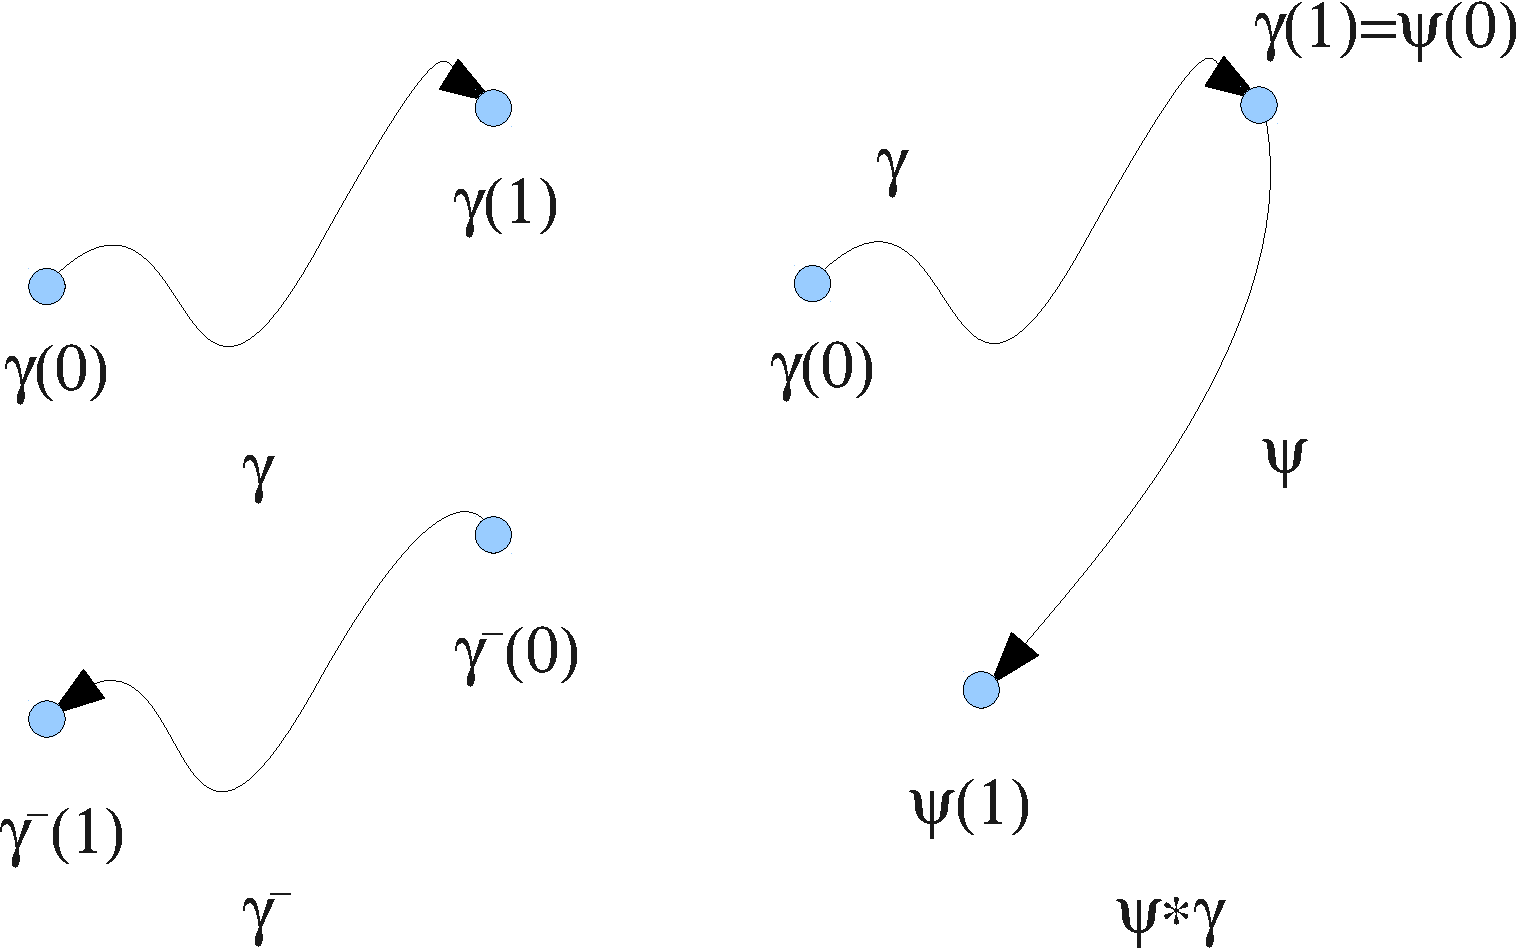
\includegraphics[scale=0.4]{images/chemins.pdf}
\caption{Chemins composé et inverse}\label{ch8:fig1}
\end{figure}

\begin{fdefn}
Un lacet $\gamma$ de $[0,1]$ dans $U$ ouvert de $\R^n$ est dit simple si, pour tout couple de points $(t_1,t_2) \in ]0,1[^2$, on a
$\gamma(t_1) \neq \gamma(t_2)$
\end{fdefn}

Il est possible de définir la longueur d'un chemin en l'approchant par des chemins polygonaux: c'est Archimède qui semble-t-il est le premier à avoir eu cette idée. La proposition suivante résume ce procédé.
\begin{fprop}
Soit $\gamma \colon [a,b] \to \R^n$ un chemin de classe $C^k$, $k \geq 1$. Pour toute subdivision $S = (a=t_0 < t_1 \dots < t_n = b)$ de l'intervalle $[a,b]$, on pose:
\[
l(S) = \sum_{i=0}^{n-1} \| \gamma(t_{i+1}) - \gamma(t_i) \|
\]
La borne supérieure de l'ensemble $\{l(S)\}$ où $S$ parcourt les subdivisions de $[a,b]$ est finie et vaut:
\[
l = \int_a^b \|\gamma^\prime(t)\| dt
\]
la valeur $l$ est appelée longueur du chemin $\gamma$.
\end{fprop}
\begin{proof}
On remarque tout d'abord, en vertu du théorème des accroissements finis que:
\[
\| \gamma(t_{i+1}) - \gamma(t_i) \|  = \left\| \int_{t_i}^{t_{i+1}} \gamma^\prime(s) ds \right\| \leq \int_{t_i}^{t_{i+1}}\left\| \gamma^\prime(s) \right\|ds
\]
on en déduit que pour toute subdivision $S$:
\[
l(S) \leq  \int_a^b \left\| \gamma^\prime(s) \right\|ds
\]
La borne supérieure de l'ensemble $l(S)$ où $S$ parcourt les subdivisions de $[a,b]$ est donc finie. Soit maintenant $\epsilon > 0$. l'application $\gamma$ étant de classe $C^1$, sa dérivée est continue sur le compact $[a,b]$, donc uniformément continue. On en déduit l'existence d'une valeur $\eta$ telle que pour toute subdivision $S =  (a=t_0 < t_1 \dots < t_n = b)$ vérifiant $\sup_{i=0}^{n-1}(t_{i+1}-t_i) < \eta$ on ait:
\[
\| \gamma^\prime(s) - \gamma^\prime(t_i)\| < \epsilon, s \in [t_i, t_{i+1}], i=0 \dots n-1
\]
Ceci implique que pour tout $i=0,\dots,n-1$:
\begin{align*}
\|\int_{t_i}^{t_{i+1}} \gamma^\prime(s) - \gamma^\prime(t_i) ds\| & = \| \gamma(t_{i+1}) - \gamma(t_i) - \gamma^\prime(t) (t_{i+1}- t_i) \| \\& < \epsilon (t_{i+1}-t_i)
\end{align*}
Soit finalement:
\[
\left| \|\gamma(t_{i+1}) - \gamma(t_i)\| -  \|\gamma^\prime(t) \|(t_{i+1}-t_i)\right | < \epsilon (t_{i+1}-t_i)
\]
On en déduit par sommation sur $i$ et application de l'inégalité triangulaire:
\[
\left|l(S) - \sum_{i=0}^n  \|\gamma^\prime(t) \|(t_{i+1}-t_i)\right| < \epsilon (b-a) 
\]
En réduisant éventuellement le pas $sup_{i=0}^{n-1}(t_{i+1}-t_i)$ des subdivisions considérées, on aura également:
\[
\left | \int_a^b \|\gamma^\prime(s)\| ds -  \sum_{i=0}^n  \|\gamma^\prime(t) \|(t_{i+1}-t_i)\right| < \epsilon (b-a) 
\]
ce qui termine la preuve. 
\end{proof}
Lorsque le chemin est de classe $C^k$ par morceaux, on définit sa longueur par sommation. 
\begin{fdefn}
Soit $\gamma \colon [a,b] \to \R^n$ un chemin de classe $C^k$ par morceaux qui est de classe $C^k$ sur chacun des intervalles $]t_i,t_{i+1}[$, où $(a=t_0 < t_1 \dots < t_n = b)$ est une subdivision de l'intervalle $[a,b]$. Sa longueur est définie par:
\[
\sum_{i=0}^{n-1} \int_{t_i}^{t_{i+1}} \| \gamma^\prime(t) \| dt
\]
\end{fdefn}
On peut montrer facilement que la longueur d'un chemin de classe $C^k$ par morceaux est encore la limite supérieure des approximations polygonales. La proposition suivante établit le fait que la longueur est un invariant géométrique d'un chemin. Elle se montre immédiatement en utilisant la formule du changement de variable dans les intégrales. 
\begin{fprop}
La longueur d'un chemin de classe $C^k$ par morceaux est invariante par changement de paramétrage.
\end{fprop}
\begin{rem}
Le procédé d'approximation par des chemins polygonaux permet de définir la longueur de chemins simplement continus, mais celle-ci peut être infinie. Lorsque la longueur est finie, on dit que le chemin est rectifiable. L'absence de formule de calcul utilisable dans le cas général fait qu'en pratique, on se restreint aux chemins de classe $C^k$ par morceaux. 
\end{rem}
\section{Intégration des formes différentielles}
\subsection{Un exemple introductif: le travail d'une force}
Le travail d'une force est en mécanique du point une notion fondamentale qui
permet de relier la variation d'énergie cinétique à l'intégrale d'une quantité
simple. Supposons donné un point matériel de masse $m$, se déplaçant dans
$\mathbb{R}^2$ et soumis à un champ de force $F \colon \mathbb{R}^2 \to
\mathbb{R}^2$ présent dans tout l'espace. En notant $\gamma \colon [a,b] \to
\mathbb{R}^2$ la trajectoire du point de l'instant $a$ à l'instant $b$, le principe fondamental
de la dynamique donne:
\[
\forall t \in ]a,b[, \, m \ddot{\gamma}(t) = F\left(\gamma(t)\right)
\]
Il est possible d'obtenir une intégrale première de cette relation en prenant le
produit scalaire avec la vitesse $\dot{\gamma}(t)$ des deux côtés de
l'égalité:
\[
\forall t \in ]a,b[, \, m \langle\ddot{\gamma}(t),\dot{\gamma}(t)\rangle =
\langle F\left(\gamma(t)\right), \dot{\gamma}(t) \rangle
\]
Comme:
\[
\frac{d\|\dot{\gamma}(t)\|^2}{dt}(t) = 2
\langle\ddot{\gamma}(t),\dot{\gamma}(t)\rangle
\]
on a, par intégration des deux membres et en supposant que la vitesse est
définie en $a$ et $b$:
\begin{equation}\label{eq:travail_force}
\frac{1}{2}m \|\dot{\gamma}(b)\|^2 - \frac{1}{2}m \|\dot{\gamma}(a)\|^2 =
\int_{[a,b]} \langle F\left(\gamma(t)\right), \dot{\gamma}(t) \rangle
dt
\end{equation}
On reconnaît en partie gauche la variation d'énergie cinétique entre $\gamma(a)$
et $\gamma(b)$, la partie droite étant le travail de la force $F$ le long du
chemin.
En règle générale, le travail dépend du chemin $\gamma$. Néanmoins, dans
certains cas, on peut montrer qu'il n'en est rien. En mécanique, ceci se produit
lorsque le champ de force dérive d'un potentiel, i.e. il existe une application
$\Psi \colon \mathbb{R}^2 \to \mathbb{R}$ telle que $F = \nabla \Psi$. On
rappelle que la notation $\nabla \Psi$ désigne le gradient de $\Psi$ qui est
défini par la relation:
\[
\forall x \in \mathbb{R}^2, \forall v \in \mathbb{R}^2, \, \langle \nabla
\Psi(x),v \rangle = \Psi^\prime(x)(v)
\]
Si l'on suppose que $F$ dérive d'un potentiel $\Psi$, le travail de $F$ s'écrit:
\begin{align*}
\int_{[a,b]} \langle F\left(\gamma(t)\right), \dot{\gamma}(t) \rangle
dt&  = \int_{[a,b]} \langle \nabla \Psi(\gamma(t)), \dot{\gamma}(t)
\rangle dt \\
&= \int_{[a,b]} \Psi^\prime(\gamma(t))(\dot{\gamma}(t)) dt \\
& = \int_{[a,b]} \frac{d}{dt}(\Psi\circ \gamma)(t) dt \\
& = \Psi\left(\gamma(b)\right) - \Psi\left(\gamma(a)\right)
\end{align*}
Cette dernière expression ne dépend plus que des points de départ et d'arrivée
et non de $\gamma$. 

L'expression de la variation de l'énergie cinétique \ref{eq:travail_force} est un exemple d'intégration d'une forme différentielle le long d'un chemin. On remarquera que la quantité $\langle F\left(\gamma(t)\right), \dot{\gamma}(t) \rangle$ exprime une projection tangentielle de $F\left(\gamma(t)\right)$ sur la courbe $\gamma$. 
\subsection{Formes différentielles}
\begin{fdefn}
Soit $U$ un ouvert de $\R^n$. On appelle forme différentielle de degré 1 et de régularité $k$ une application $\omega$ de classe $C^k$ de $U$ dans l'espace vectoriel des formes linéaires sur $\R^n$.  
\end{fdefn}
Pour un $x \in U$ fixé, $\omega(x)$ est une forme linéaire sur $\R^n$ et peut donc être appliquée à un vecteur $v \in \R^n$ pour donner un réel. On notera $\omega(x;v)$ le résultat de cette opération.

La quantité $\langle F\left(\gamma(t)\right), \dot{\gamma}(t) \rangle$ de l'exemple introductif se traduit facilement en terme de formes différentielles: il s'agit de $\omega(\gamma(t);\gamma^\prime(t))$ avec $\omega = \sum_{i=1}^2 F_i dx_i$

L'espace des formes linéaires sur $\R^n$ est canoniquement isomorphe à $\R^n$. On peut en effet prendre comme base les formes élémentaires $dx_i, i=1 \dots n$ qui à tout vecteur $v=(v_1,\dots,v_n)$ de $\R^n$ associent la $i$-ième coordonnée: $dx_i(v) = v_i$. Avec cette notation une forme différentielle $\omega$ de régularité $k$ pourra s'écrire $\omega = \sum_{i=1}^n \omega_i dx_i$ où les $\omega_i$ sont des fonctions de classe $C^k$ de $U$ dans $\R$. 
\begin{exercice}
Soit $f$ une application de classe $C^k$ définie d'un ouvert $U$ de $\R^n$ dans $\R$. Montrer que l'expression:
\[
df = \sum_{i=1}^n \frac{\partial f}{\partial x_i} dx_i
\]
définit une forme différentielle de degré 1 dont on précisera la régularité.
\end{exercice}
\begin{fdefn}
Soit $U$ un ouvert de $\R^n$. On appelle champ de vecteurs de classe $C^k$ sur $U$ une application de classe $C^k$ de $U$ dans $\R^n$. 
\end{fdefn}
De même que pour les formes différentielles, on peut écrire un champ de vecteurs en coordonnées $X(x) = (X_1(x),\dots X_n(x))$ avec $X_i, i=1 \dots n$ applications de classe $C^k$ de $U$ dans $\R$. 

Une forme différentielle de degré 1 $\omega = \sum_{i=1}^n \omega_i dx_i$ agit sur un champ de vecteurs $X$ selon la formule:
\[
x \in U \mapsto \omega(x;X(x)) = \sum_{i=1}^n \omega_i(x) X_i(x)
\]
On définit ainsi une application de $U$ dans $\R$ appelée produit contracté de $\omega$ et de $X$ et notée $(\omega | X)$. 
\begin{fdefn}
Soit $U$ ouvert de $\R^m$ et $V$ ouvert de $\R^n$. Soit $\phi \colon U \to V$ une application de classe $C^{k+1}$. A toute forme différentielle $\omega$ sur $V$ de régularité $k$ on associe une forme $\phi^*\omega$ de régularité $k$  sur $U$ définie pour tout $x$ dans $U$ et tout vecteur $v$ de $\R^m$ par la formule:
\[
\phi^*\omega(x,v) = \omega(\phi(x),\phi^\prime(x).v)
\]
La forme $\phi^*\omega$ est appelée image réciproque de $\omega$ par $\phi$.
\end{fdefn}
\begin{exercice}
En posant $\omega = \sum_{i=1}^n \omega_i dx_i$,
montrer que la forme $\phi^*\omega$ s'exprime sous la forme:
\[
\phi^*\omega = \sum_{j=1}^m \theta_j dx_j
\]
avec:
\[
\theta(x) = \phi^{\prime t} (x) \omega(\phi(x)) 
\]
où $\theta(x)$ (resp. $\omega(x)$) est le vecteur de composantes $\theta_j(x)$ (resp. $\omega_i(x)$) et $\phi^\prime(x)$ est la matrice de l'application dérivée de $\phi$ en $x$. 
\end{exercice}
L'image réciproque d'une forme différentielle s'apparente à un changement de variable. On peut procéder de même pour les champs de vecteurs, mais il s'agira ici d'une image directe.
\begin{fdefn}
Soit $U,V$ ouverts de $\R^n$. Soit $\phi \colon V \to U$ un difféomorphisme de classe $C^{k+1}$. A tout champ de vecteurs $X$ de classe $C^k$ défini sur $V$ on associe un champ de vecteurs $\phi_* X$ de classe $C^k$ sur $U$ par la formule:
\[
\phi_* X(x) = \phi^\prime(y) X(y)
\]
avec $y = \phi^{-1}(x)$.
\end{fdefn}
Contrairement à l'image réciproque d'une forme différentielle, l'image directe d'un champ de vecteurs n'est définie que pour des difféomorphismes. La proposition suivante découle directement des définitions et montre que les images directes et réciproques sont d'une certaine façon des opérations adjointes.  
\begin{prop}
Soit $U,V$ ouverts de $\R^n$. Soit $\phi \colon V \to U$ un difféomorphisme de classe $C^{k+1}$. Pour toute forme différentielle de degré 1 et de régularité $k$ sur $U$ et tout champ de vecteur de classe $C^k$ sur $V$ on a:
\[
\left(\phi^* \omega | X \right) = \left(\omega | \phi_* X \right)
\]
\end{prop}
On peut étendre la notion de forme différentielle à des degrés plus élevés:
\begin{fdefn}
Soit $U$ un ouvert de $\R^n$. On appelle forme différentielle de degré p et de régularité $k$ sur $U$ une application $\omega$ de classe $C^k$ de $U$ dans l'espace vectoriel $\Lambda^p_n$ des formes $p$-linéaires alternées sur $\R^n$. L'action au point $x$ d'une forme $\omega$ de degré $p$ sur les vecteurs $(v_1, \dots, v_p)$ sera notée $\omega(x;v_1,\dots,v_p)$. Une forme de degré 0 et de régularité $k$ sur $U$ est une application de classe $C^k$ sur $U$ à valeurs dans $\R$. 
\end{fdefn}
\begin{notation}
L'ensemble des formes différentielles de degré $p$ et de régularité $k$ sur un ouvert $U$ de $\R^n$ sera noté $\Omega_k^p(U)$.
\end{notation}
Contrairement au cas particulier $p=1$, une contrainte supplémentaire est exigée: le caractère alterné des formes linéaires. La raison de ce choix apparaîtra dans la suite lorsque on voudra interpréter une intégrale de forme comme une intégrale ordinaire.
Toute forme $p$-linéaire alternée sur $\R^n$ avec $p > n$ est identiquement nulle, on ne considérera donc que des formes de degré au plus $n$. L'espace vectoriel des formes $p$-linéaires alternées sur $\R^n$ est de dimension $C_n^p$. En effet, par la propriété de $p$-linéarité, il est suffisant de considérer l'action sur les $p$-uplets de vecteurs de base $(e_{i_1},\dots e_{i_p})$ où les indices $i_1,\dots i_p$ sont dans l'ensemble $\{1, \dots n\}$. Le caractère alterné permet de se restreindre encore aux seuls $p$-uplets $(e_{i_1},\dots e_{i_p})$ formés d'indices distincts rangés en ordre croissant, i.e. tels que $i_1 < i_2 < \dots < i_p$. On définit alors les formes $p$-alternées de base sur de tels $p$-uplets par:
\[
dx^{i_1\dots i_p}(e_{j_1},\dots,e_{j_p}) = \begin{cases}
1 \text{ si } i_1=j_1,\dots i_p=j_p \\
0 \text{ sinon }
\end{cases}
\]
\begin{fprop}
Soit $(v_1,\dots,v_p)$ un $p$-uplets de vecteurs de $\R^n$. On a:
\[
dx^{i_1\dots i_p}(v_1,\dots,v_p) = det(M) 
\]
où $M$ est la matrice $p \times p$ dont les lignes sont formées des coordonnées d'indice $i_1, \dots, i_p$ des vecteurs $v_1,\dots v_p$.
\end{fprop}
\begin{proof}
Par la $p$ linéarité et en notant $v_{jk}$ la coordonnée $k$ du vecteur $j$:
\[
dx^{i_1\dots i_p}(v_1,\dots,v_p) = \sum_{(k_1,\dots,k_p)} \prod_{j=1}^p v_{jk_j}dx^{i_1\dots i_p}(e_{k_1},\dots,e_{k_p})
\]
La définition des formes de base $dx^{i_1\dots i_p}$ montre que seuls les termes correspondant à des indices appartenant à l'ensemble $I = \{i_1, \dots , i_p\}$ sont non nuls. Il vient donc:
\[
dx^{i_1\dots i_p}(v_1,\dots,v_p) = \sum_{(k_1\in I,\dots,k_p\in I)} \prod_{j=1}^p v_{jk_j}dx^{i_1\dots i_p}(e_{k_1},\dots,e_{k_p})
\]
En utilisant le caractère alterné des formes, on peut se ramener par changement de signe au seul cas où les indices sont rangés en ordre croissant, qui donne une valeur de $1$ pour la forme de base. On en déduit l'expression:
\[
dx^{i_1\dots i_p}(v_1,\dots,v_p) = \sum_{\sigma \in \Sigma(I)} \epsilon(\sigma) \prod_{j=1}^p v_{j\sigma(i_j)}
\]
où $\Sigma(I)$ désigne l'ensemble des permutations de $I$ et $\epsilon(\sigma)$ la signature de la permutation $\sigma$. On remarque alors que cette expression est celle donnant le déterminant de la matrice $M$. 
\end{proof}
\begin{fdefn}
Un $p$-uplet d'indices $I=(i_1, \dots, i_p)$ est appelé multi-indice de longueur $p$. Il est dit ordonné si $i_1 < \dots < i_p$. La longueur d'un multi-indice $I$ est notée $|I|$.
\end{fdefn}
\begin{notation}
 Soit $I=(i_1, \dots, i_p)$ un multi-indice ordonné. On notera $dx^I$ la forme de base $dx^{i_1,\dots,i_p}$.
\end{notation}

Il est possible de définir un produit entre les formes différentielles, que l'on notera $\wedge$. 
Pour ce faire, on supposera donnés  deux multi-indices ordonnés disjoints $I=(i_1, \dots , i_p)$ et $J=(j_1, \dots j_q)$. Soit $K$ le multi-indice ordonné  $(k_1,\dots,k_{p+1})$ obtenu à partir des éléments de l'ensemble $I\cup J = \{i_1,\dots,i_p,j_1,\dots,j_q\}$. 
Il existe une unique permutation $\sigma$ associant à $(i_1,\dots,i_p,j_1,\dots,j_q)$ le multi-indice $K$. On pose:
\[
dx^I \wedge dx^J = \epsilon(\sigma) dx^K
\]
Si les deux multi-indices ordonnés $I,J$ ne sont pas disjoints, on posera $dx^I \wedge dx^J = 0$.
Un produit étant une application bilinéaire, $\wedge$ est défini de façon unique pour des formes quelconques à partir de la relation précédente. L'opération $\wedge$ est appelée produit extérieur. 
\begin{fprop}
Soient $\omega,\theta,\rho$ trois formes multilinéaires alternées de degrés respectifs $p,q,r$. On a:
\begin{enumerate}
\item $\omega \wedge \theta = (-1)^{pq} \theta \wedge \omega$.
\item $(\omega \wedge \theta) \wedge \rho = \omega \wedge (\theta \wedge \rho)$.
\item $\omega \wedge \omega = 0$.
\end{enumerate}
\end{fprop}
\begin{proof}
Il suffit de vérifier ces propriétés sur les formes de base $dx^I$, sur lesquelles elles sont immédiates.
\end{proof}
On notera que pour tout multi-indice ordonné $I=(i_1,\dots,i_p)$ on a $dx^I = dx_{i_1}\wedge \dots \wedge dx_{i_p}$.
La proposition suivante est une conséquence directe du fait que les formes $dx^I$, avec $I$ multi-indice ordonné de longueur $p$, forment une base de $\Lambda_n^p$.
\begin{fprop}
Soit $U$ un ouvert de $\R^n$. Toute forme différentielle $\omega$ de $\Omega_k^p(U)$ s'écrit de façon unique:
\[
\omega \colon x \in U \mapsto \sum_I \omega_I(x) dx^I
\]
où la somme porte sur tous les multi-indices ordonnées de longueur $p$, avec $\omega_I \colon U  \mapsto \R$ de classe $C^k$.
\end{fprop}
Le produit extérieur s'étend aux formes différentielles de la façon suivante:
\begin{fdefn}
Soit $\omega = \sum_I \omega_I dx^I$ une forme différentielle de $\Omega_k^p$ et $\theta = \sum_J \theta_J dx^J$ une forme différentielle de $\Omega_k^q$. Le produit extérieur de $\omega$ et $\theta$, noté $\omega \wedge \theta$ est défini par:
\[
\omega \wedge \theta = \sum_{I\cap J = \emptyset} \omega_I \theta_J dx^I \wedge dx^J 
\]
\end{fdefn}
Le produit extérieur des formes différentielles vérifie les mêmes propriétés que celui des formes multilinéaires alternées. 

Une forme différentielle de degré $p$ agit sur les $p$-uplets de champs de vecteurs sur $U$ selon la formule:
\[
\left(\omega|X_1,\dots,X_p\right) \colon x \in U \mapsto \omega\left(x;X_1(x),\dots,X_p(x)\right)
\]
La définition suivante est une généralisation directe de ce qui a été vu pour les formes de degré 1. 
\begin{fdefn}
Soit $U$ ouvert de $\R^m$ et $V$ ouvert de $\R^n$. Soit $\phi \colon U \to V$ une application de classe $C^{k+1}$. A toute forme différentielle $\omega$ de $\Omega_k^p(V)$ on associe une forme $\phi^*\omega$ de $\Omega_k^p(U)$ définie pour tout $x$ dans $U$ et tout $p$-uplet $v_1,\dots,v_p$ de vecteur de $\R^m$ par la formule:
\[
\phi^*\omega(x;v) = \omega(\phi(x);\phi^\prime(x).v_1,\dots,\phi^\prime(x).v_p)
\]
La forme $\phi^*\omega$ est appelée image réciproque de $\omega$ par $\phi$.
\end{fdefn}
L'image réciproque ne change pas le degré de la forme: il est donc possible qu'elle soit identiquement nulle si la dimension de l'espace de départ est trop petite. 
De même que pour les formes de degré 1, l'image réciproque des formes différentielles et l'image directe des champs de vecteurs sont des opérations adjointes. 
\begin{prop}
Soit $U,V$ ouverts de $\R^n$. Soit $\phi \colon V \to U$ un difféomorphisme de classe $C^{k+1}$. Pour toute forme différentielle de $\Omega_k^p$ et tout $p$-uplet $(X_1,\dots, X_p)$ de champs de vecteurs de classe $C^k$ sur $V$ on a:
\[
\left(\phi^* \omega | X_1,\dots X_p \right) = \left(\omega | \phi_* X_1,\dots,\phi_* X_p \right)
\]
\end{prop}
Le produit extérieur commute avec l'image réciproque:
\begin{fprop}
Soit $U$ ouvert de $\R^m$ et $V$ ouvert de $\R^n$. Soit $\phi \colon U \to V$ une application de classe $C^{k+1}$. Pour toute forme $\omega$ de $\Omega_k^p(V)$ et $\theta$ de $\Omega_k^q(V)$ on a:
\[
\phi^*(\omega \wedge \theta) = (\phi^*\omega)\wedge(\phi^*\theta)
\]
\end{fprop}
\begin{proof}
Il suffit de le vérifier sur des formes constantes $dx^I$,$dx^J$ respectivement éléments de $\Omega_k^p(V)$ et $\Omega_k^q(V)$. Soient $v_1,\dots,v_{p+q}$ des vecteurs de $\R^m$. On a, en posant comme précédemment $K$ le multi-indice ordonné obtenu à partir de $I\cup J$ et $\sigma$ la permutation ramenant $(i_1,\dots,i_p,j_1,\dots j_q)$ sur $K$:
\begin{align*}
\phi^*(dx^I \wedge dx^J)(x;v_1,\dots,v_{p+q}) & = \epsilon(\sigma) dx^K(x;\phi^\prime(x).v_1,\dots,\phi^\prime(x).v_{p+q}) \\
&  = (\phi^*dx^I)\wedge(\phi^*dx^J)(x;v_1,\dots,v_{p+q})
\end{align*}
\end{proof}
Cette proposition est très importante pour le calcul: comme toute forme de base $d^{i_1,\dots,i_p}$ peut s'écrire $dx_{i_1} \wedge \dots \wedge dx_{i_p}$, il suffit de déterminer l'image réciproque des formes de base de degré 1 pour pouvoir l'obtenir sur des formes quelconques. 


\begin{exercice}
Pour cet exercice, on se place dans l'ouvert $U = \R^2-\{(0,0)\}$. Soit la forme différentielle:
\[
\omega \colon (x,y) \mapsto dx \wedge dy
\]
\begin{itemize}
\item Montrer que l'application $\phi \colon (\rho,\theta) \mapsto (\rho \cos(\theta), \rho \sin(\theta))$ de $\R^{+*}\times [0,2\pi]$ dans $U$ est de classe $C^\infty$. Est-ce un difféomorphisme ?
\item Déterminer l'image réciproque de $\omega$ par $\phi$. 
\end{itemize}
\leftline{\textbf{Indication}:} 
On pourra dans un premier temps exprimer $\phi^*dx$ et $\phi^*dy$ en fonction de $d\rho, d\theta$ puis appliquer les propriétés du produit extérieur.
\end{exercice}

Soit $f \colon U \to \R$ de classe $C^k$ que l'on considérera comme forme de degré 0. Pour tout point $x$ de $U$, $f^\prime(x)$ est une forme linéaire sur $\R$ qui a $v$ associe le scalaire:
\[
f^\prime(x).v = \sum_{i=1}^n \frac{\partial f}{\partial x_i} v_i 
\]
elle s'identifie donc avec la forme $df = \sum_{i=1}^n \frac{\partial f}{\partial x_i} dx_i$, déjà vue en exercice. 
Soit maintenant $\omega$ une forme différentielle de $\Omega_k^p(U)$ avec $U$ ouvert de $\R^n$ et $p \geq 1$. Pour un point $x$ de $U$ donné, $\omega^\prime(x)$ est une application linéaire de $\R^n$ dans $\Lambda_n^p$, que l'on peut aussi voir comme une application multilinéaire qui a un $p+1$-uplet de vecteurs $v_1, \dots, v_{p+1}$ associe $\omega^\prime(x)(v_1)(v_2,\dots,v_{p+1})$. Cette application n'est pas alternée: le premier vecteur $v_1$ est l'argument sur lequel s'applique la dérivée en $x$ et sa permutation avec l'un des $v_i, i > 1$ n'a pas de propriété particulière. Contrairement à ce qui se passe pour les formes de degré 0, la dérivée usuelle d'une forme différentielle n'est pas une forme différentielle. Pour remédier à ce problème et obtenir une véritable dérivation, une démarche constructive va être suivie. On notera $d$ la dérivation que l'on va progressivement définir. La première hypothèse qui doit être satisfaite par $d$ est la linéarité: pour un couple de formes $\omega_1,\omega_2$ et un réel $\lambda$ quelconques, on doit avoir $d\left(\lambda \omega_1 + \omega_2 \right) = \lambda d (\omega_1) + d (\omega_2)$. Cette condition remplie, $d$ sera entièrement déterminée par ses valeurs sur des formes simples $\omega_I dx^I$ avec $I$ multi-indice quelconque et $\omega_I$ application de classe $C^k$ sur $U$ à valeurs réelles. Une forme de base $dx^I$ étant constante en tant que forme différentielle, il est naturel de poser $d(dx^I) = 0$. Par ailleurs, pour une forme simple $\omega_I dx^I$, l'application $\omega_I$ peut s'interpréter comme une forme de degré 0, conduisant à l'écriture équivalente $\omega_I \wedge dx^I$ qui ne fait plus intervenir que le produit extérieur. Finalement, il est naturel de vérifier la formule de Liebniz relative aux dérivées de produits, ce qui se traduira par:
\[
d\left(\omega_I \wedge dx^I\right) = d(\omega_I) \wedge dx^I + \omega_I \wedge d\left(dx^I\right) = d(\omega_I) \wedge dx^I
\]
Il suffit donc de définir $d$ pour les formes de degré 0 pour avoir l'expression de $d$ sur une forme quelconque. Or il a été vu plus haut que la dérivée usuelle d'une forme de degré 0 s'exprimait naturellement comme une forme différentielle de degré 1: on posera donc si $\omega$ est de degré 0:
\[
d\left(\omega\right) = \sum_{i=1}^n \frac{\partial \omega}{\partial x_i} dx_i
\]
La dérivation $d$ est entièrement définie par l'ensemble des propriété précédente. On résumera l'ensemble de la construction dans la proposition suivante:
\begin{fprop}
Il existe une unique application linéaire $d$ définie sur l'ensemble des formes différentielles de régularité $k$ sur un ouvert $U$ de $\R^n$ et à valeurs dans l'ensemble des formes différentielles de régularité $k-1$ sur $U$ vérifiant les propriétés suivantes:
\begin{enumerate}
\item Pour toute application $f$ de classe $C^k$ sur $U$ à valeurs réelles considérée comme forme de degré $0$:
\[
d\left(f\right) = \sum_{i=1}^n \frac{\partial f}{\partial x_i} dx_i
\]
\item Pour toute forme différentielle de degré $p$ $\omega = \sum_I \omega_I dx^I$, on a:
\[
d\left(\omega\right) = \sum_I d(\omega_I) \wedge dx^I
\] 
où la sommation porte sur tous les multi-indices de longueur $p$. 
\end{enumerate}
\end{fprop}
La dérivation $d$ est appelée différentielle extérieure.  Dans $\R^n$, on peut définir les formes "coordonnées" de degré 0, notées $x_1, \dots x_n$ par abus de notation et qui à tout point $y=(y_1,\dots,y_n)$ font correspondre $x_i(y) = y_i, i=1 \dots n$. On vérifie immédiatement que $d(x_i) = dx_i$, permettant ainsi d'interpréter la notation $dx_i$ comme une différentielle extérieure. 
Pour alléger les expressions, on écrira $d\omega$ au lieu de $d(\omega)$ si aucune confusion n'est possible.
\begin{fprop}
Soient $\omega, \theta$ deux formes différentielles de degrés respectifs $p$ et $q$. On a:
\[
d(\omega\wedge \theta) = d\omega \wedge \theta + (-1)^p \omega \wedge d \theta
\]
De plus, pour toute forme $\omega$ de régularité au moins 2, on a $d(d\omega) = 0$.
\end{fprop}
\begin{proof}
On notera en premier lieu que cette formule se réduit à la règle de dérivation d'un produit d'applications pour des formes de degré $0$. Par bilinéarité du produit extérieur, on peut se limiter à des formes simples $\omega_I dx^I$,$\theta_J dx^J$ avec $I$,$J$ multi-indices arbitraires. 
On a dans ce cas:
\begin{align*}
d\left(\omega\wedge \theta\right) & = d\left(\omega_I\theta_J dx^I \wedge dx^J\right) \\ & =  d\left(\omega_I\theta_J \right)\wedge dx^I \wedge dx^J \\
& = (d\omega_I \theta_J + \omega_I d \theta_J) \wedge dx^I \wedge dx^J
\end{align*}
Par ailleurs:
\[
d\omega \wedge \theta = d\omega_I \wedge dx^I \wedge dx^J
\]
et:
\[
\omega \wedge d\theta = \omega_I dx^I \wedge d\theta_J \wedge dx^J = (-1)^p \omega_I d\theta_J \wedge dx^I \wedge dx^J
\]
ce qui termine la preuve de la première partie de la proposition. 
Pour la seconde partie, on remarque tout d'abord que si $f$ est une forme de degré $0$ de régularité au moins 2, on a:
\begin{align*}
d(df) &= d \left(\sum_{i=1}^n \frac{\partial f}{\partial x_i} dx_i\right) \\
&=  \sum_{i=1}^n \sum_{j=1}^n \frac{\partial^2 f}{\partial x_j x_i} dx_j \wedge dx_i 
\end{align*}
La formule de Schwartz et l'anti-commutativité du produit extérieur donnent finalement $d(df) = 0$. Pour une forme simple $\omega_I dx_I$ de degré $p$ et de régularité au moins 2, il vient:
\[
d(d\omega) = d\left(d\omega_I \wedge dx^I\right) = d(d\omega_I)\wedge dx^I + (-1)^p \omega_I \wedge d(dx^I) = 0
\]
ce qui prouve la seconde affirmation. 
\end{proof}
\begin{notation}
Il est fréquent lors de la manipulation de formes différentielles de pouvoir former un $p-1$-uplet ordonné à partir d'un $p$-uplet ordonné. On utilise pour cela la notation suivante $(i_1,\dots,\widehat{i_k},\dots,i_p)$ pour signifier le $p-1$-uplet ordonné obtenu en supprimant la composante $k$ du $p$-uplet ordonné $(i_1,\dots,i_p)$. 
\end{notation}


L'image réciproque et la différentielle extérieure commutent:
\begin{fprop}
Soit $U$ ouvert de $\R^m$ et $V$ ouvert de $\R^n$. Soit $\phi \colon U \to V$ une application de classe $C^{k+1}$, $k > 1$. Pour toute forme $\omega$ de $\omega_k^p(V)$ on a : $d\phi^* \omega = \phi^* d \omega$
\end{fprop}
\begin{proof}
On notera dans la suite $\phi_j, j=1\dots n$ la $j$-ième composante de l'application $\phi$.
Soit $f$ application de classe $C^{k}$ sur $V$ à valeurs réelles. On a:
\begin{align*}
d \phi^* f &= \sum_{i=1}^m \frac{\partial f\circ \phi}{\partial x_i } dx_i \\
 &= \sum_{i=1}^m \sum_{j=1}^n \frac{\partial f }{\partial y_j} \frac{\partial \phi_j}{\partial x_i} dx_i \\
 & = \sum_{j=1}^n \frac{\partial f }{\partial y_j}\sum_{i=1}^m \frac{\partial \phi_j}{\partial x_i} dx_i \\
 & = \sum_{j=1}^n \frac{\partial f }{\partial y_j} d\phi_j
\end{align*}
ce qui prouve la propriété dans ce cas particulier. 
Soit maintenant une forme de base $dx^I= dx_{i_1}\wedge \dots \wedge dx_{i_p}$ de $\Omega_k^p(V)$. La règle relative à l'image réciproque d'un produit extérieur donne:
\[
\phi^* dx^I = \phi^*dx_{i_1}\wedge \dots \wedge \phi^*dx_{i_p}
\]
En appliquant la formule pour les formes de degré 0 aux formes coordonnées $x_{i_1}, \dots,x_{i_p}$ il vient:
\[
\phi^*dx_{i_1}\wedge \dots \wedge \phi^*dx_{i_p} = d \phi^* x_{i_1} \wedge \dots \wedge d\phi^*x_{i_p}
\]
on en déduit:
\[
d(\phi^* dx^I) = d\left(d \phi^* x_{i_1} \wedge \dots \wedge d\phi^*x_{i_p}\right) = 0
\]
Finalement, pour une forme simple $\omega_I dx^I$, on aura:
\begin{align*}
d\phi^*\left(\omega_I dx^I\right) & = d\left(\phi^* \omega_I \wedge \phi^* dx^I \right) \\
&= d\phi^* \omega_I \wedge \phi^* dx^I + \phi^* \omega_I \wedge d \phi^* dx^I  \\
&= \phi^* d \omega_I \wedge \phi^* dx^I = \phi^* \left(d\omega_I \wedge dx^I \right) = \phi^* d\left(\omega_I dx^I\right) 
\end{align*}
\end{proof}
Cette proposition donne un moyen très puissant de calcul pratique des images réciproques de formes différentielles. Son application conjointe avec les règles relatives au produit extérieur permet de ramener dans tous les cas le problème à une image réciproque de forme de degré 1 (ou même 0, mais cela n'apporte pas grand chose en terme de simplification). 
\subsection{Intégrale d'une 1-forme le long d'un chemin}
Cette situation sera la plus fréquente dans toute la suite. Les intégrales de chemin dans le plan complexe en seront un cas particulier. 
\begin{fdefn}
Soit $\gamma$ un chemin de classe $C^k$ par morceaux à valeurs dans un ouvert $U$ de $\R^n$. On notera $ (a=t_0 < t_1 \dots < t_n = b)$ la subdivision telle que $\gamma$ soit de classe $C^k$ sur chacun des intervalles $]t_i,t_{i+1}[, i=0,\dots,n$. Soit 
$\omega$
 une
forme différentielle de degré 1, continue sur $U$. L'intégrale de $\omega$ le long de $\gamma$ est définie comme:
\[
\int_{\gamma} \omega = \sum_{i=0}^{n-1} \int_{x_i}^{x_{i+1}} \omega\left(\gamma(t); \gamma^\prime(t)\right) dt
\]
\end{fdefn}
Dans toute la suite, on simplifiera l'écriture en ne faisant plus apparaître la somme qui devient implicite. On posera ainsi:
\[\int_{\gamma} \omega = \int_{[0,1]} \left (\alpha(\gamma(t)) dx +
\beta(\gamma(t)) dy \right). \gamma^\prime(t) dt
\]
que l'on interprétera comme une intégrale sur les morceaux $C^1$. 
On rappelle que dans l'exemple introductif sur le travail d'une force le long d'un chemin $\gamma \colon [a,b] \to \R^2$, la variation d'énergie cinétique s'exprimait comme:
\[
\int_a^n \langle F(\gamma(t)), \gamma^\prime(t) \rangle dt
\]
En notant $F_1$ (resp. $F_2$) la première (resp. seconde) composante du vecteur $F$, on remarque qu'il s'agit de l'intégrale de la forme différentielle $\omega = F_1 dx + F_2 dy$ le long de $\gamma$. D'importantes notions en physique comme le travail d'une force, le flux à travers une surface s'expriment bien à l'aide des formes différentielles et permettent souvent des écritures (et des calculs!) beaucoup plus simples. 

On remarquera que seule la continuité des formes est requise pour la définition de l'intégrale. 

\begin{exercice}
Soit $\gamma \colon t \in [0,1] \mapsto (\cos 2 \pi t, \sin 2 \pi t)$ le lacet
simple décrivant le cercle unité. Soient les deux formes différentielles
définies sur $\mathbb{R}^2$:
\[
\omega_1 =  x dx + y dy, \, \omega_2 = -y dx + x dy
\]
(on fait ici l'abus de notation classique confondant $x$ (resp. $y$) avec
l'application qui à un point $(x,y)$ associe sa coordonnée $x$ (resp. $y$)).
Calculer les intégrales de $\omega_1$ et $\omega_2$ le long de $\gamma$.
\end{exercice}
L'intégrale d'une forme différentielle possède les propriétés classiques des
intégrales.

\begin{fprop}{(Linéarité)}
Soient $\omega_1, \omega_2$ deux formes différentielles continues dans un ouvert
$U$. Soit $\gamma$ chemin de classe $C^k$ par morceaux d'image contenue dans $U$. Pour tout réel
$\lambda$ on a:
\[
\int_\gamma \lambda \omega_1 + \omega_2 = \lambda \int_\gamma \omega_1 +
\int_\gamma \omega_2
\]
\end{fprop}

La relation de Chasles sur les chemin est d'une grande importance pratique pour
le calcul explicite des intégrales.

\begin{fprop}{(Relation de Chasles)}
Soit $\omega$ une forme différentielles continue dans un ouvert
$U$. Soient $\gamma_1,\gamma_2$ chemins de classe $C^k$ par morceaux d'image contenue dans $U$.
On suppose que ces chemins sont composables. On a alors:
\begin{align*}
& \int_{\gamma_1^-} \omega = - \int_{\gamma_1} \omega \\
& \int_{\gamma_2 * \gamma_1} \omega = \int_{\gamma_1} \omega + \int_{\gamma_2}
\omega
\end{align*}
\end{fprop}

On peut étendre les intégrales de chemin à des formes différentielles à valeurs
complexes, en identifiant $\mathbb{C}$ et $\mathbb{R}^2$. On posera en pareil
cas: $dz = dx + i dy, d\overline{z} = dx - i dy$, ces deux formes constituant
une base (on peut vérifier trivialement l'indépendance linéaire). $dz,d\overline{z}$
permettent de passer d'une expression dans $\mathbb{R}^2$ à une expression dans
$\mathbb{C}$.

Si $\alpha$, $\beta$
sont des applications continues à valeurs dans $\mathbb{C}$, 
une forme différentielle $\omega$ continue s'exprimera comme:
\[
\omega = \alpha dz + \beta d\overline{z}
\]
Si $\gamma$ est un chemin de classe $C^k$ par morceaux à valeurs dans $\mathbb{C}$, et si son
image est dans le domaine de la forme $\omega$, on posera:
\begin{align*}
\int_{\gamma} \omega & = \int_{\gamma} \alpha dz + \beta d\overline{z} \\ 
& =\int_{[0,1]} (\alpha \circ \gamma)(t) \gamma^\prime(t)dt + \int_{[0,1]}
(\beta \circ \gamma)(t) \overline{\gamma^\prime}(t)dt
\end{align*}
On pourra, après séparation entre partie réelle et imaginaire, vérifier que
l'on obtient deux intégrales de chemin telles que définies dans le cadre
$\mathbb{R}^2$.
\subsection{Intégrale d'une $p$-forme sur un ouvert de $\R^p$}
C'est le second particulier qui sera vu dans le cadre de ce cours, et c'est en pratique le seul qui sera utilisé en intégration complexe, conjointement avec les intégrales de chemin. 
\begin{fdefn}
Soit $U$ un ouvert de $\R^p$ et soit $\omega = f dx_1\wedge\dots\wedge dx_p$ une forme continue de degré $p$ sur $U$. L'intégrale de $\omega$ sur $U$ est définie par:
\[
\int_U \omega = \int_U f(x) dx_1\dots dx_p
\]
l'intégrale en partie droite étant une intégrale usuelle de fonctions à valeurs réelles. 
\end{fdefn}

\subsection{Formule de Stokes}
On ne s'intéressera ici qu'au cas $\R^2$. Il existe néanmoins une formule de Stokes générale, mais qui demande l'introduction de notions assez techniques. Le lecteur qui souhaiterait approfondir ce point est invité à se reporter à un ouvrage de géométrie différentielle.  
La formule de Stokes est d'une grande importance pratique pour calculer des intégrales
de chemins à partir d'intégrales doubles, ou réciproquement. Elle sera
fondamentale pour les intégrales dans le plan complexe. 


\begin{fdefn}
Soit $U$ un ouvert de $\mathbb{R}^2$. On dira que $U$ est étoilé par rapport au
point $x \in U$ si pour tout $y \in U$ le segment de droite $[x,y]$ est contenu
dans $U$
\end{fdefn}

On notera qu'un ouvert convexe est étoilé par rapport à chacun de ses points,
mais qu'il existe des ouverts étoilés non convexes (figure \ref{ch8:fig6})
\begin{figure}[ht]
\begin{center}
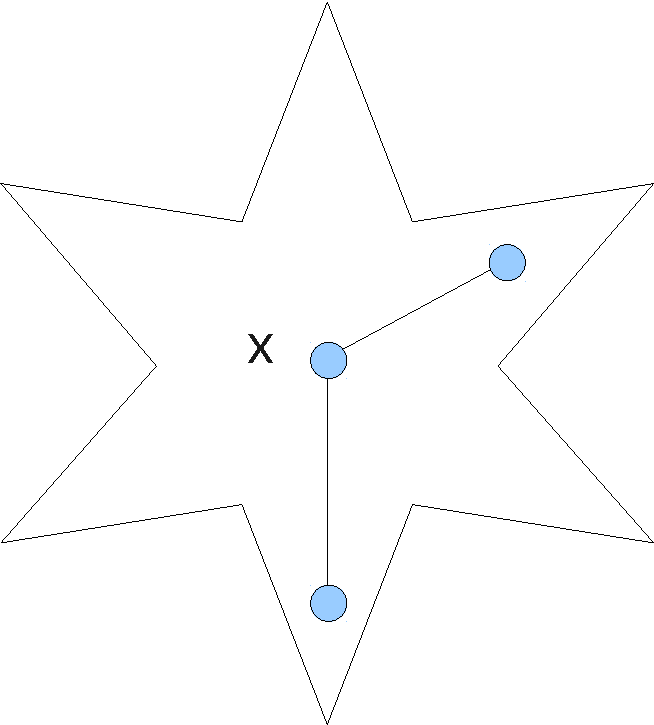
\includegraphics[scale=0.3]{images/ouvert_etoile.pdf}
\end{center}
\caption{Ouvert étoilé non convexe}\label{ch8:fig6}
\end{figure}
Une forme différentielle $f$ de degré $0$ donne par différentielle extérieure
une forme de degré 1:
\[
\omega = \frac{\partial f}{\partial x}dx + \frac{\partial f}{\partial y} dx
\]
Cette forme étant elle-même telle que $d\omega = 0$. On peut se demander s'il
existe une réciproque: si $\omega$ de degré $1$ vérifie $d\omega=0$,
peut-on trouver une fonction $f$ telle que $\omega=df$. Ceci est l'objet du
théorème de Poincaré.

\begin{fthm}
Soit $U$ un ouvert étoilé et $\omega = \alpha dx + \beta dy$ une forme de classe
$C^1$ sur $U$. Si $d\omega = 0$, il existe une forme de degré 0 sur $U$ telle
que $df = \omega$
\end{fthm}

\begin{proof}
Soit $p \in U$ un point par rapport auquel $U$ est étoilé. Soit $q$ un autre
point de $U$. On pose $v=(q-p)$ ; pour tout $t \in [0,1]$, $p + t v \in U$, on
pourra donc poser:
\[
f(p+v) = \int_{[0,1]} \alpha(p+tv).v_x + \beta(p+tv)v_y dt
\]
avec $v = v_x e_1 + v_y e_2$ ($e_1,e_2$ sont les vecteurs de base de
$\mathbb{R}^2$) En appliquant le théorème de dérivation sous le signe somme à la
fonction:
\[
h \mapsto f(p+t(v+he_1))
\]
on obtient:
\[
\frac{\partial f}{\partial x}(p+v) = \int_{[0,1]} t \frac{\partial
\alpha}{\partial x}(p+tv).v_x + \alpha(p+tv) + t \frac{\partial
\beta }{\partial x}(p+tv).v_y dt
\]
Si $d\omega = 0$, on a:
\[
\frac{\partial
\beta }{\partial x} = \frac{\partial
\alpha }{\partial y}
\]
et l'expression donnant la dérivée partielle devient:
\[
\frac{\partial f}{\partial x}(p+v) = \int_{[0,1]} t \left (\frac{\partial
\alpha}{\partial x}(p+tv).v_x +  \frac{\partial
\alpha }{\partial y}(p+tv).v_y \right) + \alpha(p+tv)  dt
\]
On a:
\[
\frac{d}{dt}\alpha(p+tv) = \left (\frac{\partial
\alpha}{\partial x}(p+tv).v_x +  \frac{\partial
\alpha }{\partial y}(p+tv).v_y \right)
\]
Et par intégration par parties:
\[
\frac{\partial f}{\partial x}(p+v) = \left[t\alpha(p+tv)\right]_0^1 =
\alpha(p+v)
\]
Prouvant bien que $\frac{\partial f}{\partial x} = \alpha$ pour tous les points
de $U$. On montrerait de même que $\frac{\partial f}{\partial x} = \beta$, ce
qui termine la preuve.
\end{proof}
Il est intéressant de noter que si l'hypothèse $d\omega =0$ n'est pas vérifiée,
on peut néanmoins construire $f$ et bien sûr calculer $df$ comme dans la preuve
précédente. Le terme résiduel qui dans ce cas rend différentes les formes $df$
et $\omega$ peut d'exprimer, avec quelques manipulations simples, uniquement en
fonction de $d\omega$, donnant en quelque sorte une généralisation du théorème.

La formule de Stokes, qui dans le cas de $\mathbb{R}^2$ porte aussi le nom de
théorème de Green-Riemann, est essentiellement une formule d'intégration par
parties pour les formes différentielles. Elle permet de transformer une
intégrale sur un ouvert de $\mathbb{R}^2$ en une intégrale sur son bord, au même
titre que la formule d'intégration par parties transforme une intégrale sur un
intervalle en une différence entre des valeurs prises sur ses extrémités.
La preuve de cette formule remarquable est délicate: les résultats présentés
ici seront volontairement limités à des cas simples, mais suffisamment généraux
pour les applications.

\begin{fprop}
Soit $U$ un ouvert de $\mathbb{R}^2$, $\Phi \colon V \to U$ un difféomorphisme
de classe $C^{k+1}$ et $\omega=\alpha dx + \beta dy$ une forme différentielle de
classe $C^k$ et de degré $1$ sur $U$. Soit enfin $\gamma$ un chemin de classe $C^1$ par morceaux
dont l'image est contenue dans $V$. On a:
\[
\int_{\Phi \circ \gamma} \omega = \int_{\gamma} \Phi^*\omega
\]
\end{fprop}

\begin{proof}
On notera encore $\Phi = \phi e_1 + \psi e_2$. 
Par définition:
\begin{align*}
\int_{\Phi \circ \gamma} \omega = & \int_{[0,1]}
\alpha\left((\Phi\circ\gamma)(t)\right) \frac{d}{dt}(\phi(\gamma(t))) \\
& + \beta\left((\Phi\circ\gamma)(t)\right) \frac{d}{dt}(\psi(\gamma(t))) dt
\end{align*}
Le théorème des fonctions composées donne, en notant $\gamma^\prime_x,
\gamma^\prime_y$ les composantes de $\gamma^\prime$ selon $e_1,e_2$:
\[
\frac{d}{dt}(\phi(\gamma(t))) = \frac{\partial \phi}{\partial
x}\gamma^\prime_x(t) + \frac{\partial \phi}{\partial
y}\gamma^\prime_y(t)
\]
et de même:
\[
\frac{d}{dt}(\psi(\gamma(t))) = \frac{\partial \psi}{\partial
x}\gamma^\prime_x(t) + \frac{\partial \psi}{\partial
y}\gamma^\prime_y(t)
\]
En regroupant les termes dans l'intégrale, on obtient:
\begin{align*}
& \int_{\Phi \circ \gamma} \omega = \\ &\int_{[0,1]}
\left(\alpha\left((\Phi\circ\gamma\right)(t)\frac{\partial \phi}{\partial
x}(t) +\beta\left((\Phi\circ\gamma\right)(t)\frac{\partial \psi}{\partial
x}(t)  + \right)\gamma^\prime_x(t) \\
& + \left(\alpha\left((\Phi\circ\gamma\right)(t)\frac{\partial \phi}{\partial
y}(t) +\beta\left((\Phi\circ\gamma\right)(t)\frac{\partial \psi}{\partial
y}(t)  + \right)\gamma^\prime_y(t) dt = \\
& \int_{\gamma} \Phi^*\omega
\end{align*}
\end{proof}

\begin{fprop}{(Théorème de Stokes élémentaire)}
Soit $\omega=\alpha dx + \beta dy$ une forme différentielle de classe $C^1$
définie sur un ouvert $U$ de $\mathbb{R}^2$, nulle en dehors d'un compact $K
\subset U$. On a:
\[
\int_{H^+} d \omega = \int_{\mathbb{R}} \alpha(x,0)dx
\]
Avec $H^+ = \mathbb{R} \times \mathbb{R}^+$ le demi-espace formé des points de
$\mathbb{R}^2$ à ordonnée positive.
\end{fprop}

\begin{proof}
La situation est résumée sur la figure \ref{ch8:fig7}. La preuve repose sur le
théorème de Fubini, et est élémentaire dans ce cas. On a par définition:
\[
d \omega = \left( \frac{- \partial \alpha }{\partial y} + \frac{\partial
\beta}{\partial x} \right) dx dy
\] 
et:
\[
\int_{H^+} d\omega = \int_{\mathbb{R}\times \mathbb{R}^+}  \left(-
\frac{\partial \alpha }{\partial y} + \frac{\partial \beta}{\partial x} \right) dxdy
\]
Le théorème de Fubini s'applique et on a:
\[
\int_{\mathbb{R}\times \mathbb{R}^+}-\frac{ \partial \alpha }{\partial
y}(x,y)dxdy = \int_{\mathbb{R}} \left(\int_{\mathbb{R}^+} -\frac{\partial \alpha
}{\partial y}(x,y)dy \right) dx
\]
Comme $\alpha$ est à support compact:
\[
\int_{\mathbb{R}^+} -\frac{\partial \alpha }{\partial
y}(x,y)dy = \alpha(x,0)
\]
De même par Fubini:
\[
\int_{\mathbb{R}\times \mathbb{R}^+}\frac{\partial \beta }{\partial
x}(x,y)dxdy = \int_{\mathbb{R}^+} \left(\int_{\mathbb{R}} \frac{\partial
\beta }{\partial x}(x,y)dx \right) dy
\]
Par compacité du support de $\beta$:
\[
\int_{\mathbb{R}} \frac{\partial
\beta }{\partial x}(x,y)dx = 0
\]
qui donne le résultat demandé.
 \begin{figure}[ht]
\begin{center}
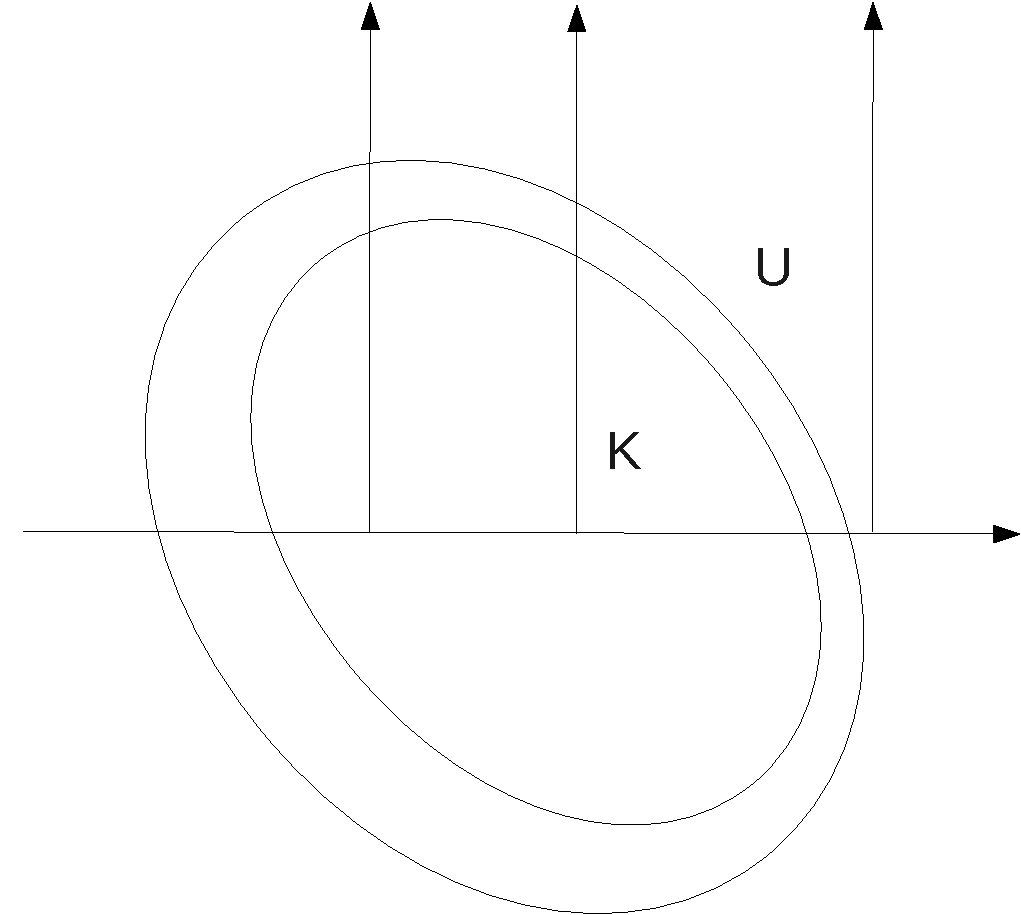
\includegraphics[scale=0.3]{images/stokes_elem.pdf}
\end{center}
\caption{Intégration de $d\omega$ par Fubini}\label{ch8:fig7}
\end{figure}
\end{proof}
On remarquera l'intégrale sur $\mathbb{R}^+$ peut être vue comme une intégrale de
chemin, en considérant pour cela un chemin correspondant à un segment de l'axe
réel et contenant le support de $\omega$.
On notera également que si le support de $\alpha$ a une intersection vide avec
l'axe réel positif, l'intégrale est nulle. Le cas général du théorème de Stokes
va s'obtenir en recollant des morceaux sur lesquels on le résultat élémentaire
pourra s'appliquer. La proposition suivante donne un procédé permettant un
découpage très régulier et s'utilise assez couramment.
\begin{fdefn}
On dira qu'un recouvrement ouvert $(U_i)_{i \in I}$ d'une partie $A \subset
\mathbb{R}^n$ est localement fini si tout point $x \in A$ possède un voisinage
ne rencontrant qu'un nombre fini d'ouverts du recouvrement.
\end{fdefn}
 \begin{fprop}{(Partitions de l'unité)}
 Soit $(U_i)_{i \in I}$ un recouvrement ouvert localement fini d'un ouvert $U
 \subset \mathbb{R}^n$. Il existe une famille d'applications $(\xi_i)_{j \in J}$ à
 valeurs dans $[0,1]$ telle que~:
 \begin{itemize}
   \item $\forall j \in J \exists i \in I \, supp(\xi_j) \subset U_i$.
   \item $\sum_{j \in J} \xi_j = 1$, où $1$ désigne l'application constante
   égale à 1.
 \end{itemize}
 \end{fprop}
La famille obtenue par la proposition précédente s'appelle partition de l'unité
subordonnée au recouvrement $(U_i)_{i \in I}$. La somme intervenant dans la
proposition est algébrique~: pour tout $x \in U$, il ne peut exister qu'un
nombre fini d'indices $j$ tels que $\xi_j(x) \neq 0$. Ceci apparaîtra clairement
au cours de la démonstration.
\begin{proof}
On remarquera tout d'abord qu'il existe une famille croissante de compacts
(pour la topologie induite sur $U$) $(K_n)_{n \in \mathbb{N}}$ telle que
$\cup_{n \in \mathbb{N}} K_n = U$ et $K_n \subset \overset{\circ}{K_{n+1}}$. Il suffit pour cela de prendre $K_n =
U \cap \overline{B(0,n)}$. Pour $n$ fixé, l'ensemble
$\tilde{K}_n = K_{n+1} - \overset{\circ}{K_{n}}$ est un compact car fermé
dans le compact $K_{n+1}$. On peut recouvrir $\tilde{K_n}$ par les ouverts
$O_{n,i} =  (\overset{\circ}{K}_{n+2} - K_{n-1}) \cap U_i$.Pour tout $x \in
O_{n,i}$, il est possible de trouver une boule ouverte $B(x,3r_x) \subset
O_{n,i}$. Soit $\psi \colon [0,1] \to [0,1]$ une application $C^\infty$ telle
que $\psi(0)=0, \psi(1)=1$ (voir le chapitre sur la transformation de Fourier
pour l'existence d'une telle fonction).
On définit $\theta_x$ par:
\[
\theta \colon y \mapsto \left \{
\begin{array}{cc}
1 & \text{ si } y \in B(x,r_x) \\
0 & \text{ si } y \in B(x,3r_x) - B(x,2r_x) \\
\psi\left(2 - \frac{\|y-x\|}{r_x}\right) & \text{ si } y \in B(x,2r_x) -
B(x,r_x)
\end{array}
\right .
\]
 Les boules ouvertes $B(x,r_x)$ forment un recouvrement ouvert du compact $\tilde{K}_n$, 
 on peut donc en extraire un sous-recouvrement fini déterminé par les points $x_{j,n}, i \in J_n$. 
 La collection $B(x_{j,n}, r_{x_{j,n}}), n \in
\mathbb{N}, j \in  J_n$ est dénombrable et vérifie les propriétés suivantes~:
\begin{itemize}
  \item Pour tout couple d'indices ${j,n}$, il existe $i \in I$ tel que
  $supp(\theta_{x_{j,n}}) \subset U_i$.
  \item Pour tout point $x \in U$, il n'existe qu'un nombre fini d'observables
  de la famille $\theta_{x_{j,n}}$ ne s'annulant pas en $x$.
  \item Pour tout point $x \in U$, il existe au moins une fonction
  de la famille $\theta_{x_{j,n}}$ ne s'annulant pas en $x$. 
\end{itemize}
Pour terminer la démonstration on pose~:
\[
\xi_{k,l} = \frac{\theta_{x_{k,l}}}{\sum_{n,j\in J_n} \theta_{x_{j,n}}} 
\]
\end{proof}

\begin{fthm}{(Théorème de Stokes)}
Soit $U$ un ouvert de $\mathbb{R}^2$ dont le bord est un lacet simple $\gamma$
de classe $C^1$ par morceaux, parcouru dans le sens trigonométrique. Soit $\omega=\alpha dx + \beta dy$ une forme différentielle
de classe $C^1$ définie sur $U$. On a: 
\[
\int_{U} d \omega = \int_{\gamma} \omega
\]
\end{fthm}

\begin{proof}
On ne donne ici qu'une idée de la preuve. Le lecteur pourra essayer de l'écrire
complètement. On supposera qu'en tout point $t$
de l'intervalle $[0,1]$, $\gamma^\prime(t) \neq 0$. En application du théorème d'inversion locale, on peut
trouver, pour tout point de $\gamma(t)$, un voisinage ouvert  $V$ de ce point et
un difféomorphisme $\Phi$ de classe $C^1$ sur un ouvert $W$ tel que
$\Phi(U\cap V) \in W\cap H^+$ et $\Phi(\gamma([0,1])\cap V)$ soit dans
l'intersection de $W$ avec l'axe réel. On peut imposer de plus
que $\Phi(\gamma(t))$ décrive un segment de l'axe réel d'abscisse croissante
avec $t$. L'image de $\gamma$ étant compacte, on peut extraire de la famille
précédente un sous-recouvrement fini. En y ajoutant l'ouvert $U$ lui-m\^eme, 
on peut construire une partition de l'unité subordonnée à cette famille. 
Sur la partie correspondant à $U$, l'intégrale de $d\omega$ est nulle.
 Sur les autres morceaux, on peut appliquer Stokes élémentaire: 
 les intégrales de chemin étant invariantes par difféomorphisme, on en déduit le
résultat.
\end{proof}
\begin{rem}
Une conséquence fondamentale du Théorème de Stokes est que l'intégrale d'une
forme fermée sur un lacet est nulle.
\end{rem}
\newpage
\leftline{\textbf{Un peu d'histoire \dots}}
\vskip 12pt
\begin{tabular}{ll}
\multicolumn{2}{l}{\textbf{Bernhard Riemann}} \\[10pt]
\begin{minipage}{0.2\linewidth}
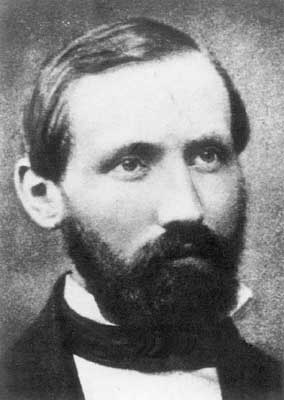
\includegraphics[scale=0.3]{images/Riemann.jpg}
\end{minipage}
&
\begin{minipage}{0.65\linewidth}
Né le  17 Septembre 1826 à Breselenz, mort le 20 Juillet 18666 à Semasca (Italie). Riemann est un des mathématiciens les plus importants de son époque et peut être de tous les temps. Durant sa courte carrière, il fonde la géométrie différentielle et contribue puissamment à l'étude des fonctions de la variable complexe. Il formalise la notion d'intégrale à partir de subdivisions de l'intervalle d'intégration.
\end{minipage}\\
\multicolumn{2}{l}{\textbf{Thomas Joannes Stieltjes}} \\[10pt]
\begin{minipage}{0.2\linewidth}
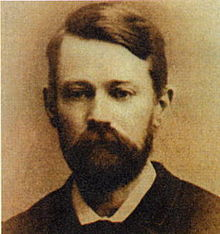
\includegraphics[scale=0.52]{images/Stieltjes.jpg}
\end{minipage}
& 
\begin{minipage}{0.65\linewidth}
Né le 29 décembre 1856 à Zwolle (Pays-Bas), mort le 31 décembre 1894 à Toulouse. Il travaillera sur les fractions continues, les formules de quadratures de Gauss et généralisera l'intégrale de Riemann.
\end{minipage}\\
\multicolumn{2}{l}{\textbf{Archimède}} \\[10pt]
\begin{minipage}{0.2\linewidth}
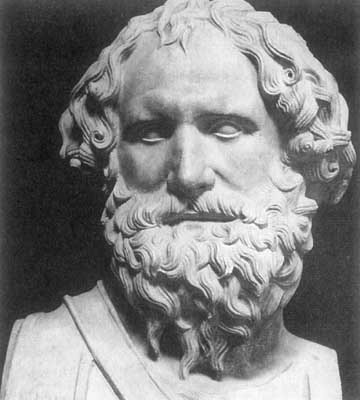
\includegraphics[scale=0.24]{images/archimede.jpg}
\end{minipage}
& 
\begin{minipage}{0.65\linewidth}
 Né à Syracuse  vers 287 av. J.-C. et mort à Syracuse en 212 av. J.-C. Génie universel, un des plus grands mathématiciens de tous les temps. Précurseur du calcul intégral, il invente la méthode d'approximation des périmètres par les chemins polygonaux. Sa défense du de Syracuse lors de son attaque par la flotte romaine et sa mort de la main d'un soldat sont particulièrement célèbres, ainsi que son exclamation "Eureka" (J'ai trouvé). On lui doit aussi l'invention de la vis, de l'écrou  et des roues dentées !
\end{minipage}\\
%\multicolumn{2}{l}{\textbf{Camille Jordan}} \\[10pt]
%\begin{minipage}{0.2\linewidth}
%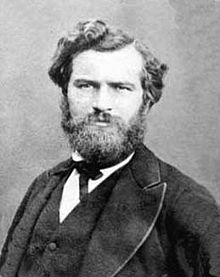
\includegraphics[scale=0.4]{images/Jordan.jpg}
%\end{minipage}
%& 
%\begin{minipage}{0.65\linewidth}
% Né à Lyon le 5 Janvier 1838 et mort à Paris le 22 Janvier 1922. Ingénieur de formation, il enseigne les mathématiques à l'école polytechnique et au collège de France. On lui doit un remarquable "cours d'analyse" ainsi que de nombreuses contributions en théorie des groupes.
%\end{minipage}
\end{tabular}
\vskip 12pt
\begin{tabular}{ll}
\multicolumn{2}{l}{\textbf{George Gabriel Stokes}} \\[10pt]
\begin{minipage}{0.2\linewidth}
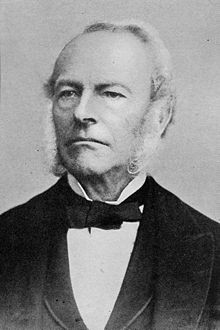
\includegraphics[scale=0.3]{images/Stokes.jpg}
\end{minipage}
&
\begin{minipage}{0.65\linewidth}
Né le  	13 août 1819 dans le Comté de Sligo (Irlande), mort le 1er février 1903 à Cambridge (Angleterre). Contribue à l'étude de la mécanique des fluide visqueux. Il explique la fluorescence de certains matériaux. Le théorème sur l'intégration des formes différentielles qui porte son nom est en réalité dû à Lord Kelvin (voir ci-dessous).
\end{minipage}\\
\multicolumn{2}{l}{\textbf{Lord Kelvin}} \\[10pt]
\begin{minipage}{0.2\linewidth}
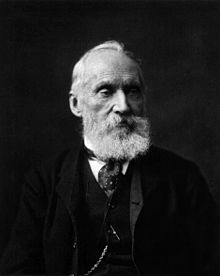
\includegraphics[scale=0.4]{images/Kelvin.jpg}
\end{minipage}
&
\begin{minipage}{0.65\linewidth}
Né le 26 juin 1824 à Belfast, mort le 17 décembre 1907 à
Largs. Physicien britannique très connu pour ses travaux en thermodynamique. On lui doit le second principe de cette science et l'échelle de température qui porte son nom. Il contribue aussi à l'électricité et à la mécanique et est un des pionniers de l'analyse vectorielle.  
\end{minipage}
\end{tabular}